\documentclass{beamer}


\usepackage{todonotes}
\usepackage{ragged2e}
\usepackage[none]{hyphenat}

\usetheme{default}
\usecolortheme{beaver}



\setbeamerfont{page number in head/foot}{size=\large}
\setbeamertemplate{footline}[frame number]
\addtobeamertemplate{block begin}{}{\justifying}

\title{Investment Value of Education in the U.S. and Europe}

\author{  
\texorpdfstring{
\begin{table}[]
\centering
\begin{tabular}{l|r}
Nathaniel Bechhofer $\star$ & \url{nbechhof@gmu.edu} \\
Omnia Elemary & \url{oelemary@gmu.edu} \\
Iman Khalil & \url{ikhalil2@gmu.edu} \\
Jaclyn Lasky & \url{jlasky2@gmu.edu} \\
Yuran (Helena) Niu & \url{yniu3@gmu.edu} \\
\end{tabular}
\end{table}
Team 4
}{People}
}

\date{\today}

\let\olditem=\item
\renewcommand{\item}{\olditem \justifying}

\begin{document}
\justify

\frame{\titlepage} % Slide 1 (title, team members, emails, team leader) 



\frame % Slide 2 Problem : Relation to Data Mining and Application/Utility; Challenges; Background
{
  \frametitle{How does education predict income?}
 \begin{block}{Problem}
  We'd like to find out how much we can infer about someone's income from their education, 
  both in the United States and Europe. 
  \end{block}
  
  \begin{block}{Why it matters}
  If income matters for variables of interest from health to happiness, we can make indirect inferences about individuals and groups using individual or average education levels \textit{combined with other information}. 
  \end{block}
  
  \begin{small}
  \begin{block}{Some motivating facts}
  \begin{itemize}
  \item \href{https://www.clevelandfed.org/newsroom-and-events/publications/economic-commentary/2012-economic-commentaries/ec-201210-the-college-wage-premium.aspx}{``College degree holders enjoy an 84 percent increase in earnings over their high-school-educated counterparts [in the United States].''} 
  \item \href{http://inequality.org/oecd-report-inequality-rising-faster/}{In the United States, income earners at the 90th percentile make roughly 16 times as much as those at the 10th percentile.}
  \item \href{http://csweb.brookings.edu/content/research/essays/2014/saving-horatio-alger.html}{Americans born in the bottom income quintile have a 10\% chance of entering the top quintile. That probability \textbf{doubles} with a college degree.}
  \end{itemize}
  \end{block}
\end{small}

}

\frame % Slide 3 
{
  \frametitle{Data Sources}
  We use two datasets, the \href{http://www.europeansocialsurvey.org/}{European Social Survey (ESS)} and the \href{https://cps.ipums.org/cps/index.shtml}{United States Current Population Survey (CPS)}; we obtained data files from the ESS website and the IPUMS (Integrated Public Use Microdata Series) in \texttt{dta} and \texttt{dat} formats.
  \begin{itemize}
  \item Both datasets are from the years 2010, 2012, and 2014.
  \item Both datasets contain rich information about respondents.
  \item We can use the US data from 2011, 2013, and 2015 to test (some of) our predictions.
  \end{itemize}
  The US data has 610,756 observations; the ESS data has 157,261 observations.
}

\frame % Slide 4
{
  \frametitle{Features}
Our dependent variable is measured differently in these datasets: the ESS gives us within country deciles, while the CPS gives a numerical answer in dollars. For the US, we only analyze those between the ages of 30 and 34 making between \$10K and \$500K. 

}




\frame % Slide 5 Architecture
{
  \frametitle{Architecture}
  \begin{itemize}
  \item For the ESS, we obtained a \texttt{dta} file with missing values and value labels already applied.
  \item We used the software Stata to apply given data definitions from IPUMS to the CPS \texttt{dat} file to obtain an informative \texttt{dta} file.  
  \item With \texttt{pandas}, a Python package, we read the \texttt{dta} files as \texttt{DataFrame} objects to use in a Python 3.5 ecosystem.
  \item Within this ecosystem, we used the \texttt{matplotlib} and \texttt{seaborn} packages for exploratory visualization.
  \end{itemize}



  
}

\frame % Slide 6
{
  \frametitle{Preprocessing}




}

\frame % Slide 7
{
  \frametitle{Normalization}


\begin{block}{Why use the natural log of income?}
  \begin{itemize}
  \item The fact that $\ln(1+x) \approx x$ enables us to think of coefficients as percentage changes.
  \item Economists typically model earnings as a function of education and work experience using the \emph{Mincer equation}, which assumes complementarity.
  \end{itemize}
  \end{block}

\begin{figure}[htbp]
\begin{center}
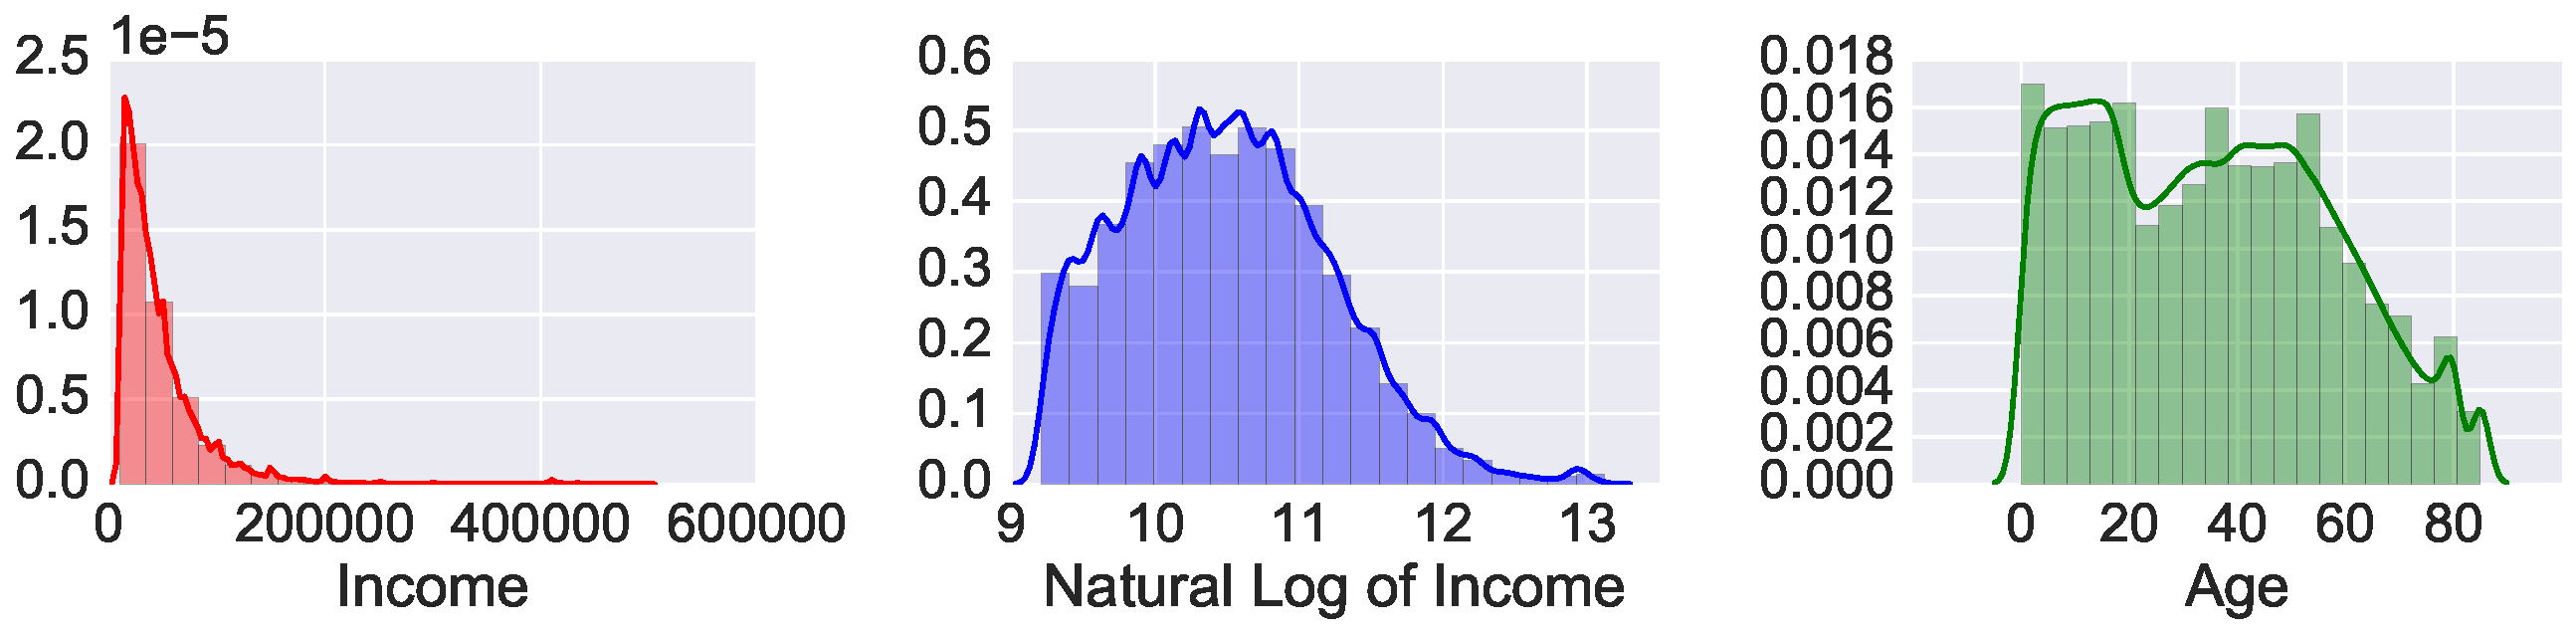
\includegraphics[width=\textwidth]{example_histograms.pdf}

\caption{Sample histograms from \texttt{seaborn}}
\label{histograms}
\end{center}
\end{figure}

}


\frame % Slide 8
{
  \frametitle{Feature Selection}
  For both data sets, we have variables telling us the following about respondents:
  \begin{itemize}
  \item Educational Attainment
  \item Age
  \item Gender
  \end{itemize}
  In addition, the European respondents consistently report parental education. 
  
  The Annual Social and Economic Supplement (ASEC) data from the CPS (obtained every March) that we are using has rich data about the occupation and employment status of respondents, which can help us clarify how education affects income.
}


\frame % Slide 9 Dimensionality Reduction
{
  \frametitle{Dimensionality Reduction}
  
 
  
  }
  

  

  



\frame % Slide 10 Model Selection
{
  \frametitle{Model Selection}

  
  
  
  }
  
  \frame % Slide 11
  {
  \frametitle{Results from Linear Regression}
  \begin{Large}
  \begin{tabular}{l*{5}{c}}
\hline\hline
\hline
College   &       1.204&       1.201&       1.327&       1.324&       0.887\\
          &    (0.0337)&    (0.0337)&    (0.0328)&    (0.0328)&    (0.0277)\\
Age         &            &      0.0383&            &      0.0402&      0.0248\\
            &            &    (0.0114)&            &    (0.0110)&   (0.00924)\\
Female         &            &            &      -1.609&      -1.609&      -0.969\\
            &            &            &    (0.0312)&    (0.0312)&    (0.0267)\\
Worker     &            &            &            &            &       4.170\\
             &            &            &            &            &    (0.0318)\\
Constant       &       8.685&       7.461&       11.10&       9.817&       1.958\\
            &    (0.0198)&     (0.364)&    (0.0506)&     (0.355)&     (0.304)\\
\hline
\(N\)       &       41254&       41254&       41254&       41254&       41254\\
adj. \(R^{2}\)&       0.030&       0.030&       0.089&       0.089&       0.357\\
\hline\hline
\multicolumn{6}{l}{\footnotesize Standard errors in parentheses}\\
\end{tabular}

  \end{Large}

\vspace{16pt}

  For all of these regression results, we have a sample size of 31640 people, all between the ages of 30 and 34 and with income between \$10000 and \$500000.
  
  }
  
  \frame % Slide 12
  {
  \frametitle{Evaluation}
  \begin{Large}
  \begin{tabular}{l*{5}{c}}
\hline\hline
\hline
College   &       1.204&       1.201&       1.327&       1.324&       0.887\\
          &    (0.0337)&    (0.0337)&    (0.0328)&    (0.0328)&    (0.0277)\\
Age         &            &      0.0383&            &      0.0402&      0.0248\\
            &            &    (0.0114)&            &    (0.0110)&   (0.00924)\\
Female         &            &            &      -1.609&      -1.609&      -0.969\\
            &            &            &    (0.0312)&    (0.0312)&    (0.0267)\\
Worker     &            &            &            &            &       4.170\\
             &            &            &            &            &    (0.0318)\\
Constant       &       8.685&       7.461&       11.10&       9.817&       1.958\\
            &    (0.0198)&     (0.364)&    (0.0506)&     (0.355)&     (0.304)\\
\hline
\(N\)       &       41254&       41254&       41254&       41254&       41254\\
adj. \(R^{2}\)&       0.030&       0.030&       0.089&       0.089&       0.357\\
\hline\hline
\multicolumn{6}{l}{\footnotesize Standard errors in parentheses}\\
\end{tabular}

  \end{Large}

\vspace{16pt}

  For all of these regression results, we have a sample size of 31640 people, all between the ages of 30 and 34 and with income between \$10000 and \$500000.
  
  }

\frame % Slide 13
{
  \frametitle{Ranked Performance}
  
}

\frame % Slide 14
{
  \frametitle{ML Algorithms}
  
}

\frame % Slide 15
{
  \frametitle{Details}
  
}
  
  
  
\frame % Slide 16 
{
  \frametitle{Prediction}
  
}

\frame % Slide 17 
{
  \frametitle{Plots}
  
}



\frame % Slide 18 Platforms (of your choice) Software and Hardware
{
  \frametitle{Platforms}
  \begin{itemize}
  \item Python 3.5
  \item \texttt{pandas} dataframe (built on \texttt{NumPy})
  \item \texttt{sci-kit learn} for ML algorithms
  \item All brought together with the Jupyter Notebook
  \item Version control using Github
  \end{itemize}
}

\frame % Slide 19 Discussion
{
  \frametitle{Discussion}

}

\frame % Slide 20 Conclusions
{
  \frametitle{Conclusion}

}



\end{document}
